%!TEX root = ../main.tex
%
% 熱電対
% レポート用紙
%

\stepcounter{section}
\section*{熱電対}

\begin{center}
\begin{tabular}{|c|c|c|c|}
\hline
\parbox[c][1.2cm][c]{0cm}{}学籍番号 & \hspace{3cm} & 名前 & \hspace{6cm} \\
\hline
\parbox[c][1.2cm][c]{0cm}{}実験日時 & \multicolumn{3}{|l|}{   年  月  日  曜日  時限}\\
\hline
\parbox[c][2.0cm][c]{0cm}{}共同実験者 & \multicolumn{3}{|l|}{}\\
\hline
\end{tabular}
\end{center}

\subsection*{実験の目的}

\vspace{5cm}

\subsection*{実験装置の全体図}


\newpage

\subsection*{測定値および計算}

\subjikken{}

\subsubsection*{冷接点の温度}
\[
\hspace*{5cm}\text{[℃]}
\]

\subsubsection*{測定値}


\hspace*{-\parindent}
\begin{tabular}{|c|c||c|c|}
\hline
水温 [℃] & 起電力 [mV] & 水温 [℃] & 起電力 [mV] \\
\hline\hline
\hspace*{3cm}&\hspace*{3cm}&\hspace*{3cm}&\hspace*{3cm}\\
\hline
&&&\\
\hline
&&&\\
\hline
&&&\\
\hline
&&&\\
\hline
&&&\\
\hline
&&&\\
\hline
&&&\\
\hline
&&&\\
\hline
&&&\\
\hline
\end{tabular}

\subsubsection*{手で暖めたときの熱起電力}
\[
\hspace*{5cm}\text{[mV]}
\]


\subsubsection*{温度差と熱起電力のグラフ}
\vspace*{1.5cm}
\hspace*{-\parindent}
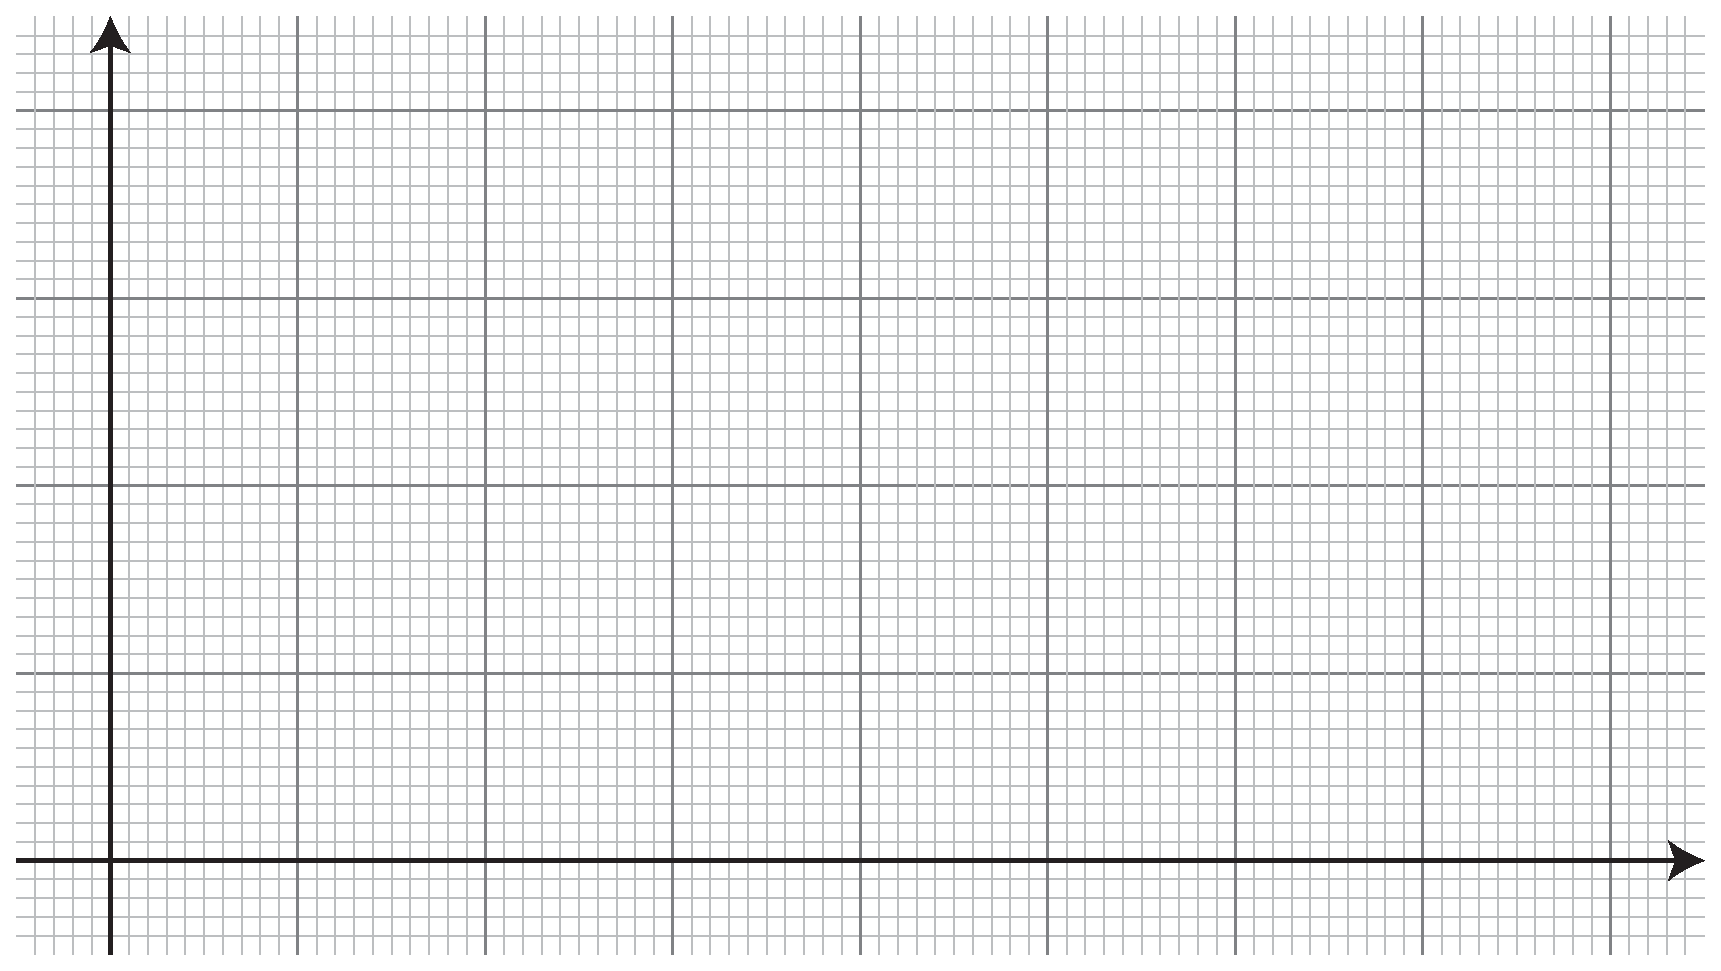
\includegraphics[scale=0.57]{10_Thermocouple/graph.eps}
\vspace*{1.5cm}


\subsubsection*{温度差$\Delta T$と熱起電力$E$の関係式}
\[
E = \fbox{\hspace{2cm}} \Delta T  +  \fbox{\hspace{2cm}} \qquad \text{(グラフより)}
\]
\[
E = \fbox{\hspace{2cm}} \Delta T  +  \fbox{\hspace{2cm}} \qquad \text{(Excelより)}
\]

\subsubsection*{体温の値}
\[
\hspace*{5cm}\text{[℃]}
\]

\newpage

\subsection*{考察}

\begin{itemize}

\item なぜ測定する部分(高温接点)とは別に、氷水で冷やした冷接点を用意する必要があるのでしょうか?

\vspace{6cm}

\item 熱電対はどのようなものに応用ができるでしょうか? また、熱電対を用いることの利点はなんでしょうか?

\end{itemize}

